% ============================================================================
%  COMPILE WITH XeLaTeX  (twice, so the point total resolves)
%  Overleaf: Menu -> Compiler -> XeLaTeX
%  Requires: bnhandout.sty and fonts/Kalpurush.ttf in the project
% ============================================================================
\documentclass[11pt]{article}
\usepackage{bnhandout}          % add [nosol] for a student edition

\hauthor[https://jugantordey.github.io]{Jugantor Dey}
\hseries{\textit{Mathematics for the Physics Olympiad}}

\begin{document}

\handouttitle{Chapter 12 : Coordinate Geometry II}

\noindent
শুরু করার আগে ৬ নম্বর অধ্যায় থেকে দূরত্বের সূত্র, ঢাল, সরলরেখা ও বৃত্তের
সমীকরণ, এবং ৭ নম্বর অধ্যায় থেকে একক বৃত্ত, radian এবং যোগ ও বিয়োগ সূত্র
ঝালিয়ে নাও। ৩ নম্বর অধ্যায়ের পূর্ণবর্গ সম্পূর্ণ করার কায়দাটিও এখানে বারবার
লাগবে।

৬ নম্বর অধ্যায়ে আমরা একটি স্থানাঙ্ক ব্যবস্থা বেছে নিয়ে তাতে জ্যামিতি
করেছিলাম। এই অধ্যায়ের মূল সুর একটু আলাদা: স্থানাঙ্ক ব্যবস্থাটি নিজেই আমাদের
পছন্দ, এবং বুদ্ধি করে বেছে নিলে একই সমস্যা অনেক সহজ হয়ে যায়। প্রথম অনুচ্ছেদে
আমরা অক্ষ সরাব ও ঘোরাব; দ্বিতীয়টিতে দেখব যে একটিমাত্র সংজ্ঞা থেকে parabola,
ellipse ও hyperbola তিনটিই বেরিয়ে আসে; তৃতীয়টিতে কার্তেসীয় অক্ষ ছেড়ে দিয়ে
কোণ ও দূরত্ব দিয়ে বিন্দু চিহ্নিত করব; আর শেষটিতে সেই ধারণাকে তিন মাত্রায় নিয়ে
যাব।

শেষ অনুচ্ছেদটি বিশেষভাবে ভবিষ্যতের জন্য। ২১ নম্বর অধ্যায়ে vector calculus
করতে গিয়ে cylindrical ও spherical স্থানাঙ্ক লাগবেই; সেগুলোর জ্যামিতিটুকু এখানে
সেরে রাখলে তখন কেবল ক্যালকুলাসটুকু করলেই চলবে। এই অধ্যায়ে মোট
\totalpoints\ পয়েন্ট আছে।

\section{অক্ষের স্থানান্তর ও ঘূর্ণন}

একটি বক্ররেখা যা, তা-ই থাকে; কিন্তু তার সমীকরণ নির্ভর করে আমরা অক্ষ কোথায়
বসিয়েছি তার উপর। তাই অক্ষ সরিয়ে বা ঘুরিয়ে সমীকরণটিকে সরল করে নেওয়া যায়।

\begin{idea}[অক্ষের স্থানান্তর]
নতুন মূলবিন্দু পুরনো ব্যবস্থার $(h,k)$ বিন্দুতে বসালে এবং অক্ষের দিক অপরিবর্তিত
রাখলে, একই বিন্দুর পুরনো স্থানাঙ্ক $(x,y)$ ও নতুন স্থানাঙ্ক $(x',y')$-এর সম্পর্ক
\[
  x' = x - h, \qquad y' = y - k ,
\]
অর্থাৎ $x = x' + h$, $y = y' + k$।
\end{idea}

চিহ্ন নিয়ে গুলিয়ে ফেলা এখানে খুব সাধারণ। মনে রাখার সহজ উপায়: নতুন মূলবিন্দু
ডান দিকে $h$ সরালে প্রতিটি বিন্দুকে নতুন ব্যবস্থায় $h$ কম দূরে মনে হবে, তাই
বিয়োগ। ১০ নম্বর অধ্যায়ে ফাংশনের লেখচিত্র সরানোর সময় ঠিক একই ব্যাপার ঘটেছিল,
কেবল সেখানে আমরা ছবিটা সরাচ্ছিলাম, এখানে অক্ষ সরাচ্ছি; দুটি একে অপরের উল্টো।

\begin{example}
$x^{2} + y^{2} - 6x + 4y - 12 = 0$ বক্ররেখাটি শনাক্ত করো এবং উপযুক্ত স্থানান্তরের
পরে তার সমীকরণ লেখো।
\end{example}

\begin{solbox}
$x$ ও $y$ আলাদা করে পূর্ণবর্গ সম্পূর্ণ করি:
\[
  (x^{2}-6x+9) + (y^{2}+4y+4) = 12 + 9 + 4
  \;\Longrightarrow\; (x-3)^{2} + (y+2)^{2} = 25 .
\]
এটি $(3,-2)$ কেন্দ্রবিশিষ্ট $5$ ব্যাসার্ধের বৃত্ত। নতুন মূলবিন্দু $(3,-2)$-এ
বসালে, অর্থাৎ $h = 3$, $k = -2$ নিলে, $x' = x-3$ ও $y' = y+2$, তাই সমীকরণ
দাঁড়ায়
\[
  x'^{2} + y'^{2} = 25 .
\]
পূর্ণবর্গ সম্পূর্ণ করা আর অক্ষ সরানো আসলে একই কাজ, দুই ভাষায় বলা।
\end{solbox}

\begin{idea}[অক্ষের ঘূর্ণন]
অক্ষ দুটিকে মূলবিন্দুর সাপেক্ষে ঘড়ির কাঁটার বিপরীতে $\theta$ কোণে ঘোরালে
\[
  x' = x\cos\theta + y\sin\theta, \qquad
  y' = -x\sin\theta + y\cos\theta ,
\]
এবং উল্টো দিকে
\[
  x = x'\cos\theta - y'\sin\theta, \qquad
  y = x'\sin\theta + y'\cos\theta .
\]
\end{idea}

\begin{center}
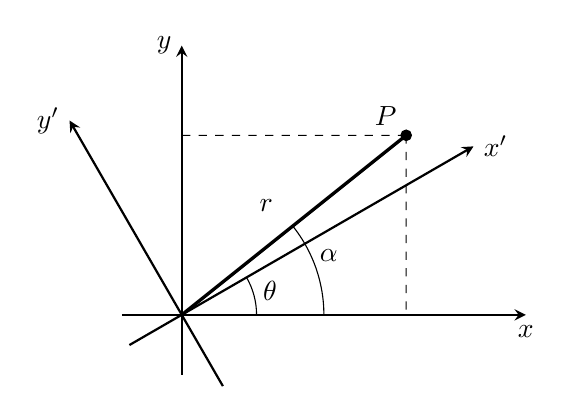
\begin{tikzpicture}[scale=0.95,>=stealth]
  \draw[thick,->] (-0.8,0) -- (4.6,0) node[below] {$x$};
  \draw[thick,->] (0,-0.8) -- (0,3.6) node[left] {$y$};
  \draw[thick,->] (-0.7,-0.404) -- (3.9,2.252) node[right] {$x'$};
  \draw[thick,->] (0.55,-0.953) -- (-1.5,2.598) node[left] {$y'$};
  \coordinate (P) at (3.0,2.4);
  \draw[very thick] (0,0) -- (P);
  \draw[fill] (P) circle (2pt) node[above left] {$P$};
  \draw[dashed] (P) -- (3.0,0); \draw[dashed] (P) -- (0,2.4);
  \draw[thin] (1.0,0) arc[start angle=0,end angle=30,radius=1.0];
  \node at (15:1.22) {$\theta$};
  \draw[thin] (1.9,0) arc[start angle=0,end angle=38.66,radius=1.9];
  \node at (22:2.12) {$\alpha$};
  \node[above left] at (1.35,1.25) {$r$};
\end{tikzpicture}
\end{center}

প্রমাণটি ৭ নম্বর অধ্যায়ের বিয়োগ সূত্র থেকে সরাসরি আসে। ধরি $P$ বিন্দুটি
মূলবিন্দু থেকে $r$ দূরে এবং পুরনো $x$-অক্ষের সঙ্গে $\alpha$ কোণে, অর্থাৎ
\[
  x = r\cos\alpha, \qquad y = r\sin\alpha .
\]
নতুন অক্ষ $\theta$ কোণে ঘোরানো, তাই নতুন ব্যবস্থায় $P$-এর কোণ $\alpha - \theta$
এবং দূরত্ব সেই একই $r$। সুতরাং
\[
  x' = r\cos(\alpha-\theta) = r\cos\alpha\cos\theta + r\sin\alpha\sin\theta
     = x\cos\theta + y\sin\theta ,
\]
\[
  y' = r\sin(\alpha-\theta) = r\sin\alpha\cos\theta - r\cos\alpha\sin\theta
     = -x\sin\theta + y\cos\theta .
\]
উল্টো সম্পর্ক দুটি একইভাবে পাওয়া যায়, কেবল $\theta$-এর জায়গায় $-\theta$ বসিয়ে।

ঘূর্ণনের সবচেয়ে বড় ব্যবহার হলো দ্বিঘাত সমীকরণ থেকে $xy$ পদটি তাড়ানো। সাধারণ
দ্বিঘাত সমীকরণ
\[
  Ax^{2} + Bxy + Cy^{2} + Dx + Ey + F = 0 .
\]
উপরের প্রতিস্থাপন বসিয়ে গুণ করলে নতুন $x'y'$ পদের সহগ দাঁড়ায়
\[
  B' = B\left( \cos^{2}\theta - \sin^{2}\theta \right)
     - 2(A-C)\sin\theta\cos\theta .
\]
৭ নম্বর অধ্যায়ের যোগ সূত্রে $B = A$ বসালেই পাওয়া যায়
$\cos 2\theta = \cos^{2}\theta - \sin^{2}\theta$ এবং
$\sin 2\theta = 2\sin\theta\cos\theta$ (এই দুটি ১৩ নম্বর অধ্যায়ে আলাদা করে
আসবে)। তাই
\[
  B' = B\cos 2\theta - (A-C)\sin 2\theta ,
\]
এবং $B' = 0$ করতে চাইলে
\[
  \cot 2\theta = \frac{A-C}{B} .
\]

\begin{example}
$xy = 1$ বক্ররেখাটি অক্ষ $45^{\circ}$ ঘুরিয়ে শনাক্ত করো।
\end{example}

\begin{solbox}
এখানে $A = C = 0$, তাই $\cot 2\theta = 0$, অর্থাৎ $2\theta = 90^{\circ}$ এবং
$\theta = 45^{\circ}$। তখন $\cos\theta = \sin\theta = 1/\sqrt{2}$, সুতরাং
\[
  x = \frac{x'-y'}{\sqrt{2}}, \qquad y = \frac{x'+y'}{\sqrt{2}} .
\]
বসিয়ে দিলে
\[
  xy = \frac{(x'-y')(x'+y')}{2} = \frac{x'^{2}-y'^{2}}{2} = 1 ,
\]
অর্থাৎ
\[
  \frac{x'^{2}}{2} - \frac{y'^{2}}{2} = 1 .
\]
এটি একটি hyperbola, যার অক্ষ পুরনো ব্যবস্থার $y = x$ রেখা বরাবর। অর্থাৎ
$xy = 1$ আর ``মান বিপরীত অনুপাতে বদলায়'' এই চেনা লেখচিত্রটি আসলে একটি
hyperbola, কেবল $45^{\circ}$ হেলানো অবস্থায় বসানো।
\end{solbox}

\prob{2} $x^{2} + 4y^{2} + 6x - 16y + 21 = 0$ সমীকরণটিকে উপযুক্ত স্থানান্তরের
মাধ্যমে সরলতম রূপে আনো এবং কেন্দ্র নির্ণয় করো।

\begin{sol}
$x$ ও $y$ আলাদা করে সাজাই:
\[
  (x^{2}+6x) + 4(y^{2}-4y) = -21 .
\]
পূর্ণবর্গ সম্পূর্ণ করে
\[
  (x+3)^{2} - 9 + 4\left[ (y-2)^{2} - 4 \right] = -21
  \;\Longrightarrow\; (x+3)^{2} + 4(y-2)^{2} = 4 .
\]
$h = -3$, $k = 2$ নিয়ে $x' = x+3$, $y' = y-2$ বসালে
\[
  \frac{x'^{2}}{4} + y'^{2} = 1 .
\]
কেন্দ্র $(-3, 2)$। খেয়াল করো, $4$ দিয়ে গুণ করা বন্ধনীর ভেতরে $-4$ ঢুকলে বাইরে
$-16$ হয়; এই জায়গাটাতেই সবচেয়ে বেশি ভুল হয়।
\end{sol}

\prob{2} অক্ষকে $30^{\circ}$ ঘোরানো হলো। $(x,y) = (\sqrt{3},\,1)$ বিন্দুটির নতুন
স্থানাঙ্ক নির্ণয় করো এবং ফলটি ব্যাখ্যা করো।

\begin{sol}
$\cos 30^{\circ} = \sqrt{3}/2$ ও $\sin 30^{\circ} = 1/2$ বসিয়ে
\[
  x' = \sqrt{3}\cdot\frac{\sqrt{3}}{2} + 1\cdot\frac{1}{2}
     = \frac{3}{2} + \frac{1}{2} = 2 ,
\]
\[
  y' = -\sqrt{3}\cdot\frac{1}{2} + 1\cdot\frac{\sqrt{3}}{2} = 0 .
\]
সুতরাং নতুন স্থানাঙ্ক $(2,0)$।

ব্যাখ্যা: বিন্দুটির মূলবিন্দু থেকে দূরত্ব $\sqrt{3+1} = 2$ এবং $x$-অক্ষের সঙ্গে
তার কোণ $\arctan(1/\sqrt{3}) = 30^{\circ}$। অক্ষকেও ঠিক $30^{\circ}$ ঘোরানো
হয়েছে, তাই বিন্দুটি নতুন $x'$-অক্ষের উপরেই পড়ে গেছে; সেজন্য $y' = 0$ আর
$x'$ হলো ওই দূরত্বটাই।
\end{sol}

\prob{3} অক্ষ $\theta$ কোণে ঘোরানো হলে দেখাও যে
$x'^{2} + y'^{2} = x^{2} + y^{2}$। এখান থেকে দেখাও যে দুটি বিন্দুর মধ্যেকার
দূরত্ব ঘূর্ণনে বদলায় না।

\begin{sol}
সংক্ষেপে $c = \cos\theta$, $s = \sin\theta$ লিখি। তাহলে
\[
  x'^{2} + y'^{2} = (xc+ys)^{2} + (-xs+yc)^{2} .
\]
খুলে লিখি:
\[
  = x^{2}c^{2} + 2xycs + y^{2}s^{2} + x^{2}s^{2} - 2xycs + y^{2}c^{2}
  = x^{2}(c^{2}+s^{2}) + y^{2}(c^{2}+s^{2}) .
\]
আড়াআড়ি পদ দুটি কাটাকাটি গেছে, আর $c^{2}+s^{2} = 1$ (৭ নম্বর অধ্যায়)।
সুতরাং $x'^{2}+y'^{2} = x^{2}+y^{2}$।

দূরত্বের জন্য: দুটি বিন্দু $P_{1}, P_{2}$ নিলে ঘূর্ণনের সূত্রগুলো রৈখিক, তাই
\[
  x'_{2} - x'_{1} = (x_{2}-x_{1})c + (y_{2}-y_{1})s, \qquad
  y'_{2} - y'_{1} = -(x_{2}-x_{1})s + (y_{2}-y_{1})c .
\]
অর্থাৎ পার্থক্য দুটিও একই ঘূর্ণন মানে। উপরের ফল ওদের উপর প্রয়োগ করলে
\[
  (x'_{2}-x'_{1})^{2} + (y'_{2}-y'_{1})^{2} = (x_{2}-x_{1})^{2} + (y_{2}-y_{1})^{2} ,
\]
অর্থাৎ দূরত্ব অপরিবর্তিত। এটি অবশ্য অবাক করার মতো নয়; অক্ষ ঘোরালে বিন্দুগুলো তো
নড়েনি, কেবল তাদের নাম বদলেছে। কিন্তু বীজগণিত থেকেও যে একই কথা বেরোয়, সেটা
দেখে নেওয়া ভালো।
\end{sol}

\section{কনিক}

\begin{idea}[Focus, directrix ও eccentricity]
একটি বিন্দু $F$ (focus), একটি সরলরেখা $d$ (directrix, যা $F$-এর মধ্য দিয়ে যায়
না) এবং একটি ধনাত্মক সংখ্যা $e$ (eccentricity) নাও। যেসব বিন্দু $P$-এর জন্য
\[
  PF = e \cdot \operatorname{dist}(P, d) ,
\]
তাদের সমষ্টিকে বলে conic। $e < 1$ হলে ellipse, $e = 1$ হলে parabola, $e > 1$
হলে hyperbola।
\end{idea}

তিনটি আলাদা বক্ররেখা নয়, একটিই পরিবার; কেবল $e$ সংখ্যাটি বদলায়। এই একত্রিত
দৃষ্টিভঙ্গিটাই তৃতীয় অনুচ্ছেদে সবচেয়ে বেশি কাজে দেবে।

\begin{center}
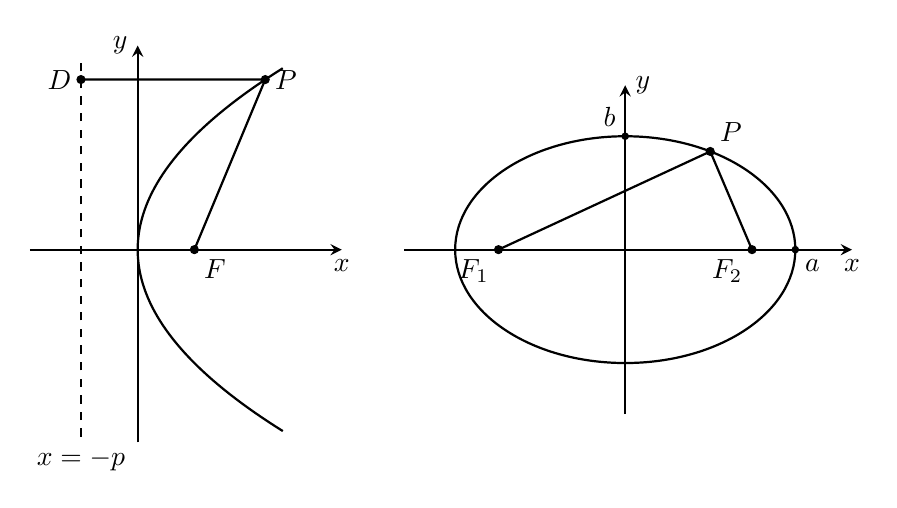
\begin{tikzpicture}[scale=0.72,>=stealth]
 \begin{scope}
  \draw[thick,->] (-1.9,0) -- (3.6,0) node[below] {$x$};
  \draw[thick,->] (0,-3.4) -- (0,3.6) node[left] {$y$};
  \draw[thick,domain=-3.2:3.2,samples=80,variable=\t] plot ({\t*\t/4},{\t});
  \draw[thick,dashed] (-1,-3.3) -- (-1,3.3);
  \node[below] at (-1,-3.35) {$x=-p$};
  \draw[fill] (1,0) circle (2pt) node[below right] {$F$};
  \coordinate (P) at (2.25,3);
  \draw[fill] (P) circle (2pt) node[right] {$P$};
  \draw[thick] (1,0) -- (P);
  \draw[thick] (P) -- (-1,3);
  \draw[fill] (-1,3) circle (2pt) node[left] {$D$};
 \end{scope}
 \begin{scope}[xshift=8.6cm]
  \draw[thick,->] (-3.9,0) -- (4.0,0) node[below] {$x$};
  \draw[thick,->] (0,-2.9) -- (0,2.9) node[right] {$y$};
  \draw[thick] (0,0) ellipse (3 and 2);
  \draw[fill] (2.236,0) circle (2pt) node[below left] {$F_{2}$};
  \draw[fill] (-2.236,0) circle (2pt) node[below left] {$F_{1}$};
  \coordinate (Q) at (1.5,1.732);
  \draw[fill] (Q) circle (2pt) node[above right] {$P$};
  \draw[thick] (-2.236,0) -- (Q) -- (2.236,0);
  \draw[fill] (3,0) circle (1.6pt) node[below right] {$a$};
  \draw[fill] (0,2) circle (1.6pt) node[above left] {$b$};
 \end{scope}
\end{tikzpicture}
\end{center}

$e = 1$ ক্ষেত্রটি দিয়ে শুরু করি, কারণ সেটি সবচেয়ে সহজ। Focus $(p,0)$ এবং
directrix $x = -p$ নিলে শর্তটি দাঁড়ায়
\[
  \sqrt{(x-p)^{2}+y^{2}} = x + p .
\]
দুই পাশ বর্গ করে
\[
  x^{2} - 2px + p^{2} + y^{2} = x^{2} + 2px + p^{2}
  \;\Longrightarrow\; y^{2} = 4px .
\]
এটিই parabola-র আদর্শ রূপ। $p > 0$ হলে সে ডানে খোলে, $p < 0$ হলে বামে।

এবার $e \neq 1$। Focus $(ae, 0)$ এবং directrix $x = a/e$ নিই, যেখানে $a > 0$
একটি ধ্রুবক (কেন এই বিশেষ পছন্দ, তা এক্ষুনি পরিষ্কার হবে)। শর্তটি
\[
  \sqrt{(x-ae)^{2}+y^{2}} = e\left( \frac{a}{e} - x \right) = a - ex .
\]
বর্গ করে
\[
  x^{2} - 2aex + a^{2}e^{2} + y^{2} = a^{2} - 2aex + e^{2}x^{2} ,
\]
অর্থাৎ $x^{2}\left( 1 - e^{2} \right) + y^{2} = a^{2}\left( 1-e^{2} \right)$।
$a^{2}(1-e^{2})$ দিয়ে ভাগ করে
\[
  \frac{x^{2}}{a^{2}} + \frac{y^{2}}{a^{2}\left( 1-e^{2} \right)} = 1 .
\]

\begin{idea}[Ellipse ও hyperbola-র আদর্শ রূপ]
$e < 1$ হলে $b^{2} = a^{2}(1-e^{2}) > 0$ ধরে
\[
  \frac{x^{2}}{a^{2}} + \frac{y^{2}}{b^{2}} = 1
  \qquad (\mathrm{ellipse}, \ a > b) ,
\]
এবং $e > 1$ হলে $b^{2} = a^{2}(e^{2}-1) > 0$ ধরে
\[
  \frac{x^{2}}{a^{2}} - \frac{y^{2}}{b^{2}} = 1
  \qquad (\mathrm{hyperbola}) .
\]
দুই ক্ষেত্রেই $c = ae$ লিখলে focus $(\pm c, 0)$, এবং
\[
  c^{2} = a^{2} - b^{2} \ (\mathrm{ellipse}), \qquad
  c^{2} = a^{2} + b^{2} \ (\mathrm{hyperbola}), \qquad
  e = \frac{c}{a} .
\]
Hyperbola-র asymptote দুটি $y = \pm \dfrac{b}{a} x$।
\end{idea}

$a$-কে ওভাবে বেছে নেওয়ার কারণটা এবার দেখা যাচ্ছে: ellipse-এর ক্ষেত্রে $x = \pm a$
বিন্দু দুটিই বক্ররেখার দুই প্রান্ত, তাই $a$ হলো অর্ধ-বৃহৎ অক্ষ।

উপরের হিসাবের মাঝপথে একটি ফল লুকিয়ে আছে, যা আলাদা করে তুলে রাখার মতো। শর্তটি
লেখার সময়ই আমরা পেয়েছি
\[
  PF_{2} = a - ex ,
\]
যেখানে $F_{2} = (ae, 0)$। প্রতিসাম্যের কারণে বাম দিকের focus $F_{1} = (-ae,0)$
ও তার directrix $x = -a/e$ নিলে একইভাবে $PF_{1} = a + ex$। যোগ করলে
\[
  PF_{1} + PF_{2} = 2a .
\]
অর্থাৎ ellipse-এর যেকোনো বিন্দু থেকে দুই focus-এর দূরত্বের যোগফল ধ্রুবক। এটিই
সেই চেনা সুতোর কৌশল: দুটি পিন পুঁতে সুতো টান টান রেখে পেন্সিল ঘোরালে ellipse
আঁকা হয়। Hyperbola-র ক্ষেত্রে একই হিসাব দেয় $|PF_{1} - PF_{2}| = 2a$, যোগফলের
বদলে বিয়োগফল।

\begin{idea}[সাধারণ দ্বিঘাত সমীকরণ চেনা]
$Ax^{2} + Bxy + Cy^{2} + Dx + Ey + F = 0$ সমীকরণটি (অবক্ষয়ী ক্ষেত্র বাদে)
\[
  B^{2} - 4AC < 0 \ \Rightarrow \ \mathrm{ellipse}, \qquad
  B^{2} - 4AC = 0 \ \Rightarrow \ \mathrm{parabola}, \qquad
  B^{2} - 4AC > 0 \ \Rightarrow \ \mathrm{hyperbola} .
\]
\end{idea}

কেন এটি কাজ করে? কারণ $B^{2}-4AC$ রাশিটি অক্ষের ঘূর্ণন ও স্থানান্তরে বদলায় না।
এই অপরিবর্তনীয়তা এখানে প্রমাণ করা হচ্ছে না, ধরে নেওয়া হচ্ছে; তবে ইচ্ছা করলে
আগের অনুচ্ছেদের প্রতিস্থাপন বসিয়ে হাতে যাচাই করা যায়, কেবল হিসাবটা লম্বা।
অবক্ষয়ী ক্ষেত্র বলতে বোঝানো হচ্ছে সেসব ক্ষেত্র, যেখানে সমীকরণটি একটি বিন্দু,
এক জোড়া সরলরেখা, বা কিছুই না বোঝায়; যেমন $x^{2}+y^{2} = 0$।

\begin{example}
$9x^{2} + 4y^{2} - 18x + 16y - 11 = 0$ শনাক্ত করো এবং তার কেন্দ্র, $a$, $b$,
focus ও eccentricity নির্ণয় করো।
\end{example}

\begin{solbox}
$B = 0$ এবং $B^{2}-4AC = -144 < 0$, তাই ellipse আশা করছি। পূর্ণবর্গ সম্পূর্ণ
করি:
\[
  9(x^{2}-2x) + 4(y^{2}+4y) = 11
  \;\Longrightarrow\; 9(x-1)^{2} - 9 + 4(y+2)^{2} - 16 = 11 ,
\]
অর্থাৎ $9(x-1)^{2} + 4(y+2)^{2} = 36$, এবং $36$ দিয়ে ভাগ করে
\[
  \frac{(x-1)^{2}}{4} + \frac{(y+2)^{2}}{9} = 1 .
\]
কেন্দ্র $(1,-2)$। বড় হরটি $y$-এর নিচে, তাই বৃহৎ অক্ষ উল্লম্ব: $a = 3$ (উল্লম্ব
দিকে), $b = 2$। সুতরাং
\[
  c = \sqrt{a^{2}-b^{2}} = \sqrt{5}, \qquad e = \frac{c}{a} = \frac{\sqrt{5}}{3}
  \approx 0.745 .
\]
Focus দুটি কেন্দ্র থেকে উল্লম্বভাবে $\sqrt{5}$ দূরে, অর্থাৎ
$\left( 1,\, -2 \pm \sqrt{5} \right)$।
\end{solbox}

\prob{2} $y^{2} = -12x$ parabola-টির focus, directrix ও অক্ষ নির্ণয় করো, এবং
সে কোন দিকে খোলে তা বলো।

\begin{sol}
আদর্শ রূপ $y^{2} = 4px$-এর সঙ্গে মিলিয়ে $4p = -12$, অর্থাৎ $p = -3$।

Focus $(p, 0) = (-3, 0)$; directrix $x = -p$, অর্থাৎ $x = 3$; অক্ষ হলো
$x$-অক্ষ। $p < 0$ বলে parabola-টি বাম দিকে খোলে, যা $y^{2} = -12x$ থেকেও স্পষ্ট,
কারণ ডান পাশ অঋণাত্মক হতে $x \leq 0$ লাগে।
\end{sol}

\prob{2} $4x^{2} + 9y^{2} - 8x + 36y + 4 = 0$ শনাক্ত করো এবং কেন্দ্র, $a$, $b$,
focus ও eccentricity নির্ণয় করো।

\begin{sol}
\[
  4(x^{2}-2x) + 9(y^{2}+4y) = -4
  \;\Longrightarrow\; 4(x-1)^{2} - 4 + 9(y+2)^{2} - 36 = -4 ,
\]
অর্থাৎ $4(x-1)^{2} + 9(y+2)^{2} = 36$, তাই
\[
  \frac{(x-1)^{2}}{9} + \frac{(y+2)^{2}}{4} = 1 .
\]
কেন্দ্র $(1,-2)$; এবার বড় হরটি $x$-এর নিচে, তাই বৃহৎ অক্ষ অনুভূমিক, $a = 3$,
$b = 2$, $c = \sqrt{9-4} = \sqrt{5}$, $e = \sqrt{5}/3$। Focus দুটি
$\left( 1 \pm \sqrt{5},\, -2 \right)$।
\end{sol}

\prob{3} $\dfrac{x^{2}}{a^{2}} - \dfrac{y^{2}}{b^{2}} = 1$ hyperbola-র জন্য
দেখাও যে $x$ বড় হলে বক্ররেখাটি $y = \dfrac{b}{a}x$ রেখার যত কাছে ইচ্ছা চলে যায়,
কিন্তু কখনো তাকে ছোঁয় না।

\begin{sol}
প্রথম চতুর্ভাগে সমীকরণ থেকে
$y = \dfrac{b}{a}\sqrt{x^{2}-a^{2}}$ (যেখানে $x \geq a$)। রেখা ও বক্ররেখার
উল্লম্ব ব্যবধান
\[
  \frac{b}{a}x - y = \frac{b}{a}\left( x - \sqrt{x^{2}-a^{2}} \right) .
\]
লব ও হরে $x + \sqrt{x^{2}-a^{2}}$ দিয়ে গুণ করি (৩ নম্বর অধ্যায়ের
$(u-v)(u+v) = u^{2}-v^{2}$):
\[
  \frac{b}{a}\left( x - \sqrt{x^{2}-a^{2}} \right)
  = \frac{b}{a} \cdot \frac{x^{2} - (x^{2}-a^{2})}{x + \sqrt{x^{2}-a^{2}}}
  = \frac{ab}{x + \sqrt{x^{2}-a^{2}}} .
\]
হরটি $x$-এর সঙ্গে বাড়ে এবং যত ইচ্ছা বড় হতে পারে, তাই গোটা ভগ্নাংশটি $0$-এর যত
কাছে ইচ্ছা যায়। আবার লব $ab$ ধনাত্মক এবং হর সসীম, তাই ভগ্নাংশটি কখনো ঠিক $0$
হয় না; অর্থাৎ ছোঁয়া হয় না।

``যত কাছে ইচ্ছা যায়'' কথাটির নির্ভুল রূপ limit, যা ১৪ নম্বর অধ্যায়ের বিষয়;
এখানে বীজগণিত দিয়েই ব্যাপারটা দেখা গেল।
\end{sol}

\prob{3} $5x^{2} - 6xy + 5y^{2} - 8 = 0$ বক্ররেখাটি ঘূর্ণন ব্যবহার করে শনাক্ত
করো এবং তার $a$ ও $b$ নির্ণয় করো।

\begin{sol}
$A = C = 5$, তাই $\cot 2\theta = (A-C)/B = 0$, অর্থাৎ $\theta = 45^{\circ}$।
বসাই
\[
  x = \frac{x'-y'}{\sqrt{2}}, \qquad y = \frac{x'+y'}{\sqrt{2}} .
\]
তাহলে
\[
  5x^{2} + 5y^{2} = \frac{5}{2}\left[ (x'-y')^{2} + (x'+y')^{2} \right]
  = 5\left( x'^{2} + y'^{2} \right) ,
\]
\[
  -6xy = -\frac{6}{2}\left( x'^{2} - y'^{2} \right) = -3x'^{2} + 3y'^{2} .
\]
যোগ করে $2x'^{2} + 8y'^{2} = 8$, অর্থাৎ
\[
  \frac{x'^{2}}{4} + y'^{2} = 1 .
\]
এটি একটি ellipse, যার $a = 2$ (নতুন $x'$-অক্ষ বরাবর, অর্থাৎ পুরনো ব্যবস্থার
$y = x$ রেখা বরাবর) এবং $b = 1$। যাচাই: $B^{2}-4AC = 36 - 100 = -64 < 0$, যা
ellipse-ই বলছিল।
\end{sol}

\section{পোলার স্থানাঙ্ক}

কোনো বিন্দু চিহ্নিত করার আরেকটি স্বাভাবিক উপায় হলো বলা: মূলবিন্দু থেকে কত দূরে,
আর কোন দিকে। এটিই polar coordinate, এবং বৃত্তীয় প্রতিসাম্য থাকলে এতে কাজ অনেক
সহজ হয়।

\begin{idea}[Polar coordinate]
বিন্দু $P$-এর polar coordinate $(r, \theta)$, যেখানে $r$ হলো মূলবিন্দু থেকে
দূরত্ব এবং $\theta$ হলো ধনাত্মক $x$-অক্ষ থেকে ঘড়ির কাঁটার বিপরীতে মাপা কোণ।
সম্পর্কগুলো
\[
  x = r\cos\theta, \qquad y = r\sin\theta ,
\]
\[
  r = \sqrt{x^{2}+y^{2}}, \qquad
  \cos\theta = \frac{x}{r}, \qquad \sin\theta = \frac{y}{r} .
\]
এই সিরিজে আমরা সবসময় $r \geq 0$ ধরব।
\end{idea}

\begin{center}
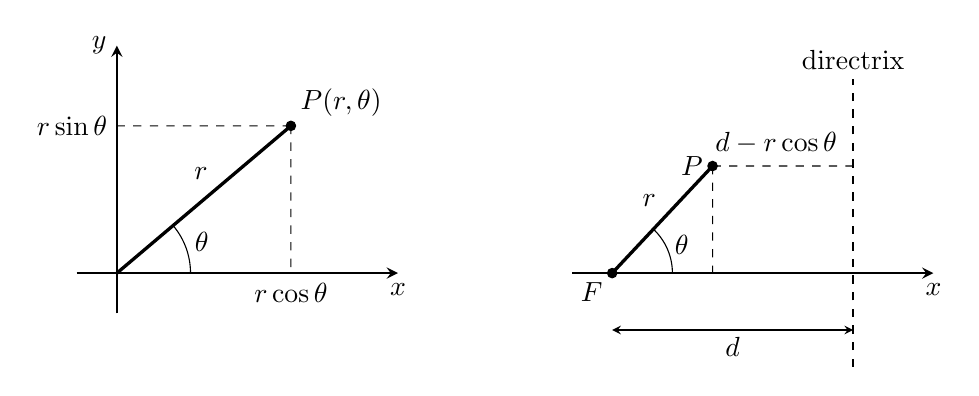
\begin{tikzpicture}[scale=0.85,>=stealth]
 \begin{scope}
  \draw[thick,->] (-0.6,0) -- (4.2,0) node[below] {$x$};
  \draw[thick,->] (0,-0.6) -- (0,3.4) node[left] {$y$};
  \coordinate (P) at (2.6,2.2);
  \draw[very thick] (0,0) -- (P);
  \draw[fill] (P) circle (2pt) node[above right] {$P(r,\theta)$};
  \draw[dashed] (P) -- (2.6,0) node[below] {$r\cos\theta$};
  \draw[dashed] (P) -- (0,2.2) node[left] {$r\sin\theta$};
  \draw[thin] (1.1,0) arc[start angle=0,end angle=40.2,radius=1.1];
  \node at (20:1.35) {$\theta$};
  \node[above left] at (1.5,1.25) {$r$};
 \end{scope}
 \begin{scope}[xshift=7.4cm]
  \draw[thick,->] (-0.6,0) -- (4.8,0) node[below] {$x$};
  \draw[thick,dashed] (3.6,-1.4) -- (3.6,2.9);
  \node[above] at (3.6,2.9) {directrix};
  \coordinate (P) at (1.5,1.6);
  \draw[fill] (0,0) circle (2pt) node[below left] {$F$};
  \draw[very thick] (0,0) -- (P);
  \draw[fill] (P) circle (2pt) node[left] {$P$};
  \draw[dashed] (P) -- (3.6,1.6);
  \draw[dashed] (P) -- (1.5,0);
  \draw[thin] (0.9,0) arc[start angle=0,end angle=46.8,radius=0.9];
  \node at (22:1.12) {$\theta$};
  \node[above left] at (0.8,0.85) {$r$};
  \draw[<->] (0,-0.85) -- (3.6,-0.85); \node[below] at (1.8,-0.82) {$d$};
  \node[above] at (2.45,1.63) {$d-r\cos\theta$};
 \end{scope}
\end{tikzpicture}
\end{center}

\begin{remark}
$r \geq 0$ শর্তটি একটি পছন্দ, সর্বজনীন নিয়ম নয়। অনেক ক্যালকুলাস বইয়ে $r$
ঋণাত্মকও হতে দেওয়া হয়, যেখানে $(-r, \theta)$ মানে $(r, \theta+\pi)$ বিন্দুটি।
পদার্থবিজ্ঞানে দূরত্ব ঋণাত্মক হয় না, তাই আমরা $r \geq 0$-ই রাখছি। এর একটি
ফল আছে যা খেয়াল রাখতে হবে: $r = f(\theta)$ ধরনের বক্ররেখা কেবল সেসব $\theta$-তে
সংজ্ঞায়িত, যেখানে $f(\theta) \geq 0$। একই বক্ররেখার সমীকরণ তাই দুই নিয়মে দুই
রকম বস্তু বোঝাতে পারে, আর সেটাই এই অনুচ্ছেদের শেষ সমস্যাটির বিষয়।

আরেকটি ছোট কথা: $(r,\theta)$ আর $(r, \theta + 2\pi)$ একই বিন্দু, তাই polar
coordinate এক-এক নয়। মূলবিন্দুতে $r = 0$ এবং $\theta$ অনির্ধারিত।
\end{remark}

\begin{idea}[কয়েকটি চেনা বক্ররেখা]
\begin{enumerate}
  \item $r = a$ (ধ্রুবক) হলো মূলবিন্দু-কেন্দ্রিক $a$ ব্যাসার্ধের বৃত্ত।
  \item $\theta = \alpha$ (ধ্রুবক) হলো মূলবিন্দু থেকে বেরোনো একটি রশ্মি, পুরো
        সরলরেখা নয়, কারণ $r \geq 0$।
  \item $r = 2a\cos\theta$ হলো $(a, 0)$ কেন্দ্রবিশিষ্ট $a$ ব্যাসার্ধের বৃত্ত,
        যা মূলবিন্দু দিয়ে যায়।
\end{enumerate}
\end{idea}

তৃতীয়টি দেখা সহজ। দুই পাশকে $r$ দিয়ে গুণ করে
\[
  r^{2} = 2ar\cos\theta
  \;\Longrightarrow\; x^{2}+y^{2} = 2ax
  \;\Longrightarrow\; (x-a)^{2} + y^{2} = a^{2} .
\]
$r$ দিয়ে গুণ করার ধাপটি মূলবিন্দুতে ($r=0$) বাড়তি একটি সমাধান ঢোকাতে পারে,
কিন্তু এখানে মূলবিন্দু এমনিতেই বক্ররেখার উপরে ($\theta = \pi/2$-তে $r=0$), তাই
কোনো ক্ষতি নেই।

\begin{example}
$x^{2}+y^{2} = 4x$ বৃত্তটিকে polar আকারে লেখো, এবং $r = 3\sin\theta$-কে
কার্তেসীয় আকারে লিখে শনাক্ত করো।
\end{example}

\begin{solbox}
প্রথমটি: $x^{2}+y^{2} = r^{2}$ ও $x = r\cos\theta$ বসিয়ে
$r^{2} = 4r\cos\theta$, অর্থাৎ $r = 4\cos\theta$ (এবং $r=0$, যা এই বক্ররেখারই
একটি বিন্দু)।

দ্বিতীয়টি: দুই পাশকে $r$ দিয়ে গুণ করে $r^{2} = 3r\sin\theta$, অর্থাৎ
\[
  x^{2}+y^{2} = 3y
  \;\Longrightarrow\; x^{2} + \left( y - \tfrac{3}{2} \right)^{2} = \tfrac{9}{4} .
\]
এটি $(0, 3/2)$ কেন্দ্রবিশিষ্ট $3/2$ ব্যাসার্ধের বৃত্ত, যা মূলবিন্দু স্পর্শ করে
এবং $y$-অক্ষের উপর বসানো।
\end{solbox}

\begin{idea}[Conic-এর polar সমীকরণ]
Focus মূলবিন্দুতে এবং directrix $x = d$ ($d > 0$) রেখায় বসালে eccentricity $e$
বিশিষ্ট conic-এর সমীকরণ
\[
  r = \frac{ed}{1 + e\cos\theta} .
\]
\end{idea}

প্রমাণটি ছবির ডান পাশ থেকে এক লাইনে আসে। $P$ বিন্দুর focus থেকে দূরত্ব $r$, আর
directrix থেকে দূরত্ব $d - r\cos\theta$। সংজ্ঞা বলছে
\[
  r = e\left( d - r\cos\theta \right)
  \;\Longrightarrow\; r\left( 1 + e\cos\theta \right) = ed
  \;\Longrightarrow\; r = \frac{ed}{1+e\cos\theta} .
\]
Directrix বাম পাশে ($x = -d$) বসালে হরে চিহ্নটি বিয়োগ হয়ে যায়, আর directrix
অনুভূমিক হলে $\cos$-এর জায়গায় $\sin$ আসে।

এই একটিমাত্র সমীকরণে তিনটি conic-ই ধরা আছে, এবং focus মূলবিন্দুতে বসানো বলে
এটিই সেই রূপ যা পদার্থবিজ্ঞানে দরকার হয়।

\begin{example}
$r = \dfrac{6}{1 + \tfrac{1}{2}\cos\theta}$ বক্ররেখাটি শনাক্ত করো এবং তার
$e$, $d$, focus থেকে নিকটতম ও দূরতম দূরত্ব, এবং $a$ নির্ণয় করো।
\end{example}

\begin{solbox}
আদর্শ রূপের সঙ্গে মিলিয়ে $e = \tfrac{1}{2}$ এবং $ed = 6$, তাই $d = 12$।
$e < 1$, সুতরাং এটি একটি ellipse যার একটি focus মূলবিন্দুতে।

$\cos\theta$-এর মান $-1$ থেকে $1$ পর্যন্ত যায়, তাই হর সবচেয়ে বড় হয়
$\theta = 0$-তে এবং সবচেয়ে ছোট হয় $\theta = \pi$-তে:
\[
  r_{\min} = \frac{6}{1+\tfrac{1}{2}} = 4, \qquad
  r_{\max} = \frac{6}{1-\tfrac{1}{2}} = 12 .
\]
এই দুটি হলো বৃহৎ অক্ষের দুই প্রান্ত, তাই $2a = 4 + 12 = 16$, অর্থাৎ $a = 8$।
তারপর $c = ae = 4$ এবং $b = a\sqrt{1-e^{2}} = 8 \cdot \tfrac{\sqrt{3}}{2}
= 4\sqrt{3}$। যাচাই: $a - c = 8 - 4 = 4 = r_{\min}$, মিলে যাচ্ছে।
\end{solbox}

\begin{remark}
গ্রহের কক্ষপথ ঠিক এই আকারের: সূর্য একটি focus-এ, আর কক্ষপথ একটি conic যার
$e$ কক্ষপথের চ্যাপ্টা ভাব ঠিক করে। পৃথিবীর জন্য $e \approx 0.017$, অর্থাৎ প্রায়
বৃত্ত; ধূমকেতুর জন্য $e$ প্রায় $1$, তাই সে লম্বা সরু পথে আসে আর যায়। উপরের
$r_{\min}$ ও $r_{\max}$ হলো সূর্যের নিকটতম ও দূরতম বিন্দু।

কেন বর্গ-বিপরীত আকর্ষণ থেকে ঠিক এই বক্ররেখাগুলোই বেরোয়, সেটি এখানে দেখানো
যাচ্ছে না; তার জন্য differential equation লাগে, যা ১৯ নম্বর অধ্যায়ের বিষয়।
এখানে কেবল এটুকু জেনে রাখো যে যন্ত্রপাতিটা তৈরি হয়ে গেল।
\end{remark}

\prob{2} নিচেরগুলোকে polar আকারে লেখো এবং শনাক্ত করো।
\begin{enumerate}
  \item $x^{2}+y^{2} = 9$
  \item $y = x$
  \item $x^{2}+y^{2}-6y = 0$
\end{enumerate}

\begin{sol}
\begin{enumerate}
  \item $r^{2} = 9$, অর্থাৎ $r = 3$ (কারণ $r \geq 0$); মূলবিন্দু-কেন্দ্রিক
        $3$ ব্যাসার্ধের বৃত্ত।
  \item $r\sin\theta = r\cos\theta$, অর্থাৎ $\tan\theta = 1$। $r \geq 0$ ধরায়
        $\theta = \pi/4$ কেবল প্রথম চতুর্ভাগের রশ্মিটি দেয়; পুরো সরলরেখা পেতে
        হলে $\theta = \pi/4$ এবং $\theta = 5\pi/4$ দুটিই লাগবে।
  \item $r^{2} = 6r\sin\theta$, অর্থাৎ $r = 6\sin\theta$; $(0,3)$
        কেন্দ্রবিশিষ্ট $3$ ব্যাসার্ধের বৃত্ত।
\end{enumerate}
\end{sol}

\prob{2} $r = 4\sin\theta + 2\cos\theta$ বক্ররেখাটিকে কার্তেসীয় আকারে লিখে
শনাক্ত করো।

\begin{sol}
দুই পাশকে $r$ দিয়ে গুণ করি:
\[
  r^{2} = 4r\sin\theta + 2r\cos\theta
  \;\Longrightarrow\; x^{2}+y^{2} = 4y + 2x .
\]
পূর্ণবর্গ সম্পূর্ণ করে
\[
  (x-1)^{2} + (y-2)^{2} = 1 + 4 = 5 .
\]
$(1,2)$ কেন্দ্রবিশিষ্ট $\sqrt{5}$ ব্যাসার্ধের বৃত্ত, যা মূলবিন্দু দিয়ে যায়
(যাচাই: $1 + 4 = 5$)।
\end{sol}

\prob{3} $r = \dfrac{8}{3 + \cos\theta}$ বক্ররেখাটি শনাক্ত করো এবং $e$, $d$,
$a$, $b$, $c$ এবং focus থেকে নিকটতম ও দূরতম দূরত্ব নির্ণয় করো।

\begin{sol}
আদর্শ রূপে আনতে লব ও হরকে $3$ দিয়ে ভাগ করি:
\[
  r = \frac{8/3}{1 + \tfrac{1}{3}\cos\theta} .
\]
সুতরাং $e = \tfrac{1}{3}$ এবং $ed = \tfrac{8}{3}$, অর্থাৎ $d = 8$। $e<1$, তাই
ellipse।
\[
  r_{\min} = \frac{8/3}{1+\tfrac{1}{3}} = 2, \qquad
  r_{\max} = \frac{8/3}{1-\tfrac{1}{3}} = 4 .
\]
$2a = 2 + 4 = 6$, তাই $a = 3$; $c = ae = 1$; এবং
$b = \sqrt{a^{2}-c^{2}} = \sqrt{8} = 2\sqrt{2}$।
যাচাই: $a - c = 2 = r_{\min}$ এবং $a + c = 4 = r_{\max}$।
\end{sol}

\prob{3} $r = 4\cos 2\theta$ বক্ররেখাটি $r \geq 0$ নিয়মে বিবেচনা করো। কোন কোন
$\theta$-তে এটি সংজ্ঞায়িত, এবং লেখচিত্রে কয়টি পাপড়ি থাকবে? $r$ ঋণাত্মক হতে
দিলে উত্তর কীভাবে বদলাত?

\begin{sol}
$r \geq 0$ লাগবে, অর্থাৎ $\cos 2\theta \geq 0$। এটি ঘটে যখন
\[
  2\theta \in \left[ -\tfrac{\pi}{2}, \tfrac{\pi}{2} \right]
  \qquad \text{or} \qquad
  2\theta \in \left[ \tfrac{3\pi}{2}, \tfrac{5\pi}{2} \right] ,
\]
অর্থাৎ
\[
  \theta \in \left[ -\tfrac{\pi}{4}, \tfrac{\pi}{4} \right]
  \qquad \text{or} \qquad
  \theta \in \left[ \tfrac{3\pi}{4}, \tfrac{5\pi}{4} \right] .
\]
প্রতিটি ব্যবধিতে $r$ প্রান্তে $0$ থেকে শুরু হয়ে মাঝখানে সর্বোচ্চ $4$ হয়ে আবার
$0$-তে ফেরে, অর্থাৎ একটি করে পাপড়ি। সুতরাং পাপড়ির সংখ্যা দুই: একটি
$\theta = 0$ ঘিরে ($x$-অক্ষের ধনাত্মক দিকে) এবং একটি $\theta = \pi$ ঘিরে।

$r$ ঋণাত্মক হতে দিলে বাদ পড়া ব্যবধি দুটিও আঁকা যেত, এবং সেখানকার বিন্দুগুলো
বসত $y$-অক্ষ বরাবর। তখন মোট চারটি পাপড়ি পাওয়া যেত। একই সমীকরণ, অথচ দুই নিয়মে
দুই রকম ছবি; এই কারণেই নিয়মটা আগে থেকে ঠিক করে নেওয়া জরুরি।
\end{sol}

\section{অন্যান্য বক্ররৈখিক স্থানাঙ্ক}

তিন মাত্রায় polar-এর দুটি স্বাভাবিক সম্প্রসারণ আছে, আর কোনটি বেছে নেবে তা ঠিক
করে দেয় সমস্যার প্রতিসাম্য: অক্ষ-প্রতিসাম্য হলে cylindrical, বিন্দু-প্রতিসাম্য
হলে spherical।

\begin{idea}[Cylindrical coordinate $(s, \phi, z)$]
$s$ হলো $z$-অক্ষ থেকে বিন্দুটির লম্ব দূরত্ব, $\phi$ হলো ধনাত্মক $x$-অক্ষ থেকে
$xy$-সমতলে মাপা কোণ, আর $z$ যথারীতি উচ্চতা। এখানে $s \geq 0$ এবং
$0 \leq \phi < 2\pi$।
\[
  x = s\cos\phi, \qquad y = s\sin\phi, \qquad z = z ,
\]
\[
  s = \sqrt{x^{2}+y^{2}}, \qquad \tan\phi = \frac{y}{x} .
\]
\end{idea}

\begin{idea}[Spherical coordinate $(r, \theta, \phi)$]
$r$ হলো মূলবিন্দু থেকে দূরত্ব, $\theta$ হলো ধনাত্মক $z$-অক্ষ থেকে মাপা কোণ
(polar angle), আর $\phi$ হলো আগের মতোই $xy$-সমতলে মাপা কোণ (azimuthal angle)।
এখানে $r \geq 0$, $0 \leq \theta \leq \pi$, $0 \leq \phi < 2\pi$।
\[
  x = r\sin\theta\cos\phi, \qquad
  y = r\sin\theta\sin\phi, \qquad
  z = r\cos\theta ,
\]
\[
  r = \sqrt{x^{2}+y^{2}+z^{2}}, \qquad
  \cos\theta = \frac{z}{r}, \qquad
  \tan\phi = \frac{y}{x} .
\]
\end{idea}

\begin{center}
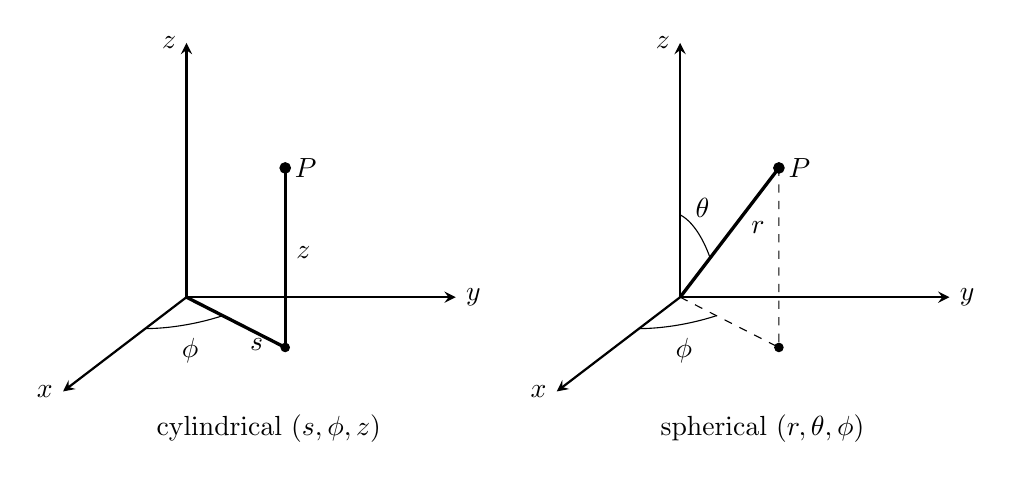
\begin{tikzpicture}[scale=0.95,>=stealth]
 \begin{scope}
  \draw[thick,->] (0,0) -- (-1.65,-1.26) node[left] {$x$};
  \draw[thick,->] (0,0) -- (3.6,0) node[right] {$y$};
  \draw[thick,->] (0,0) -- (0,3.4) node[left] {$z$};
  \coordinate (P) at (1.32,1.728);
  \coordinate (Q) at (1.32,-0.672);
  \draw[very thick] (0,0) -- (Q); \draw[very thick] (Q) -- (P);
  \draw[fill] (P) circle (2pt) node[right] {$P$};
  \draw[fill] (Q) circle (1.6pt);
  \draw[thin,domain=0:54,samples=40,variable=\a]
       plot ({1.0*(cos(\a)*(-0.55)+sin(\a))},{1.0*(cos(\a)*(-0.42))});
  \node at (0.05,-0.72) {$\phi$};
  \node[below right] at (0.72,-0.42) {$s$};
  \node[right] at (1.34,0.6) {$z$};
  \node at (1.1,-1.75) {cylindrical $(s,\phi,z)$};
 \end{scope}
 \begin{scope}[xshift=6.6cm]
  \draw[thick,->] (0,0) -- (-1.65,-1.26) node[left] {$x$};
  \draw[thick,->] (0,0) -- (3.6,0) node[right] {$y$};
  \draw[thick,->] (0,0) -- (0,3.4) node[left] {$z$};
  \coordinate (P) at (1.32,1.728);
  \coordinate (Q) at (1.32,-0.672);
  \draw[very thick] (0,0) -- (P);
  \draw[dashed] (0,0) -- (Q) -- (P);
  \draw[fill] (P) circle (2pt) node[right] {$P$};
  \draw[fill] (Q) circle (1.6pt);
  \draw[thin,domain=0:54,samples=40,variable=\a]
       plot ({1.0*(cos(\a)*(-0.55)+sin(\a))},{1.0*(cos(\a)*(-0.42))});
  \node at (0.05,-0.72) {$\phi$};
  \draw[thin,domain=0:48.6,samples=40,variable=\b]
       plot ({0.534*sin(\b)},{-0.2717*sin(\b)+1.1*cos(\b)});
  \node at (0.30,1.20) {$\theta$};
  \node[below right] at (0.82,1.14) {$r$};
  \node at (1.1,-1.75) {spherical $(r,\theta,\phi)$};
 \end{scope}
\end{tikzpicture}
\end{center}

Spherical সূত্র তিনটি মুখস্থ করার দরকার নেই, ছবি থেকে দুই ধাপে বেরিয়ে আসে।
$P$ থেকে $z$-অক্ষের উপর লম্ব ফেলো। যে সমকোণী ত্রিভুজ হয় তার অতিভুজ $r$ এবং
$z$-অক্ষের সঙ্গে কোণ $\theta$, তাই
\[
  z = r\cos\theta, \qquad s = r\sin\theta .
\]
এবার $xy$-সমতলে নেমে এসো: সেখানে $P$-এর ছায়া মূলবিন্দু থেকে $s$ দূরে এবং
$x$-অক্ষের সঙ্গে $\phi$ কোণে, তাই আগের অনুচ্ছেদের polar সূত্র অনুযায়ী
$x = s\cos\phi$ ও $y = s\sin\phi$। এখানে $s$-এর জায়গায় $r\sin\theta$ বসিয়ে
দিলেই তিনটি সূত্র পাওয়া গেল।

\begin{idea}[ধ্রুবক স্থানাঙ্কের তল]
\begin{enumerate}
  \item $s = s_{0}$: $z$-অক্ষ ঘিরে $s_{0}$ ব্যাসার্ধের cylinder।
  \item $\phi = \phi_{0}$: $z$-অক্ষে কব্জা লাগানো একটি অর্ধ-সমতল।
  \item $r = r_{0}$: মূলবিন্দু-কেন্দ্রিক $r_{0}$ ব্যাসার্ধের গোলক।
  \item $\theta = \theta_{0}$: মূলবিন্দুতে শীর্ষবিন্দুবিশিষ্ট একটি অর্ধ-cone,
        যার অক্ষ $z$-অক্ষ। বিশেষ ক্ষেত্রে $\theta_{0} = \pi/2$ দেয়
        $xy$-সমতল।
\end{enumerate}
\end{idea}

\begin{remark}
এখানে একটি সতর্কবার্তা, এবং এটি সত্যিই গুরুত্বপূর্ণ। গণিতের বইয়ে (এই সিরিজের
সহায়ক বইগুলো সহ) spherical coordinate লেখা হয় $(\rho, \theta, \phi)$ আকারে,
যেখানে $\theta$ হলো azimuthal কোণ আর $\phi$ হলো $z$-অক্ষ থেকে মাপা কোণ; অর্থাৎ
আমাদের $\theta$ ও $\phi$-এর ভূমিকা ঠিক উল্টো, আর দূরত্বকে বলা হয় $\rho$।
পদার্থবিজ্ঞানে প্রায় সর্বত্র (এবং ২১ নম্বর অধ্যায়ে) উপরের নিয়মটিই চলে, তাই
এই সিরিজ সেটিকেই ধরছে। বই বদলালে প্রথমেই ছবি দেখে যাচাই করে নাও কোন অক্ষর কোন
কোণ বোঝাচ্ছে; নাহলে একটি sine আর একটি cosine অদলবদল হয়ে গোটা হিসাব ভুল হয়ে
যাবে।

দ্বিতীয় ছোট কথা: দ্বিমাত্রিক polar coordinate-এ আমরা কোণটিকে $\theta$ বলেছি,
যেটি তিন মাত্রায় গিয়ে $\phi$ হয়ে গেল। এটি অসংগতি নয়, প্রচলিত অভ্যাস; সমতলে
কোণ একটাই, তাই তার নাম নিয়ে বিভ্রান্তির সুযোগ নেই।
\end{remark}

\begin{remark}
ভূগোলের সঙ্গে মিলিয়ে নিলে $\theta$ মনে রাখা সহজ। $\phi$ হলো দ্রাঘিমাংশ
(longitude), আর $\theta$ হলো উত্তর মেরু থেকে মাপা কোণ, অর্থাৎ অক্ষাংশ নয়
বরং তার পরিপূরক; অক্ষাংশকে $\lambda$ ধরলে $\theta = 90^{\circ} - \lambda$। উত্তর মেরুতে
$\theta = 0$, বিষুবরেখায় $\theta = 90^{\circ}$, দক্ষিণ মেরুতে
$\theta = 180^{\circ}$।
\end{remark}

\begin{example}
\begin{enumerate}
  \item $(x,y,z) = \left( 0,\, 2,\, 2\sqrt{3} \right)$ বিন্দুটির spherical
        স্থানাঙ্ক নির্ণয় করো।
  \item $z = \sqrt{x^{2}+y^{2}}$ তলটিকে spherical স্থানাঙ্কে প্রকাশ করো।
\end{enumerate}
\end{example}

\begin{solbox}
(১) $r = \sqrt{0 + 4 + 12} = 4$। তারপর
$\cos\theta = z/r = 2\sqrt{3}/4 = \sqrt{3}/2$, অর্থাৎ $\theta = 30^{\circ}$।
$xy$-সমতলে ছায়াটি $(0,2)$, যা ধনাত্মক $y$-অক্ষের উপর, তাই
$\phi = 90^{\circ}$। সুতরাং $(r,\theta,\phi) = (4,\, 30^{\circ},\, 90^{\circ})$।

যাচাই: $x = 4\sin 30^{\circ}\cos 90^{\circ} = 0$,
$y = 4\sin 30^{\circ}\sin 90^{\circ} = 2$,
$z = 4\cos 30^{\circ} = 2\sqrt{3}$।

(২) $\sqrt{x^{2}+y^{2}} = s = r\sin\theta$ এবং $z = r\cos\theta$, তাই শর্তটি
দাঁড়ায় $r\cos\theta = r\sin\theta$। মূলবিন্দু বাদে $r > 0$, তাই
$\tan\theta = 1$, অর্থাৎ
\[
  \theta = \frac{\pi}{4} .
\]
অর্থাৎ তলটি একটি অর্ধ-cone, যা ঠিক ধ্রুবক-$\theta$ তলের উদাহরণ। কার্তেসীয়
আকারে এটি চেনা কঠিন ছিল, spherical-এ একটিমাত্র সমীকরণ।
\end{solbox}

\prob{2} \begin{enumerate}
  \item $(x,y,z) = \left( 1,\, 1,\, \sqrt{2} \right)$-এর spherical স্থানাঙ্ক
        নির্ণয় করো।
  \item $(r,\theta,\phi) = \left( 6,\, 60^{\circ},\, 120^{\circ} \right)$-এর
        কার্তেসীয় স্থানাঙ্ক নির্ণয় করো।
\end{enumerate}

\begin{sol}
\begin{enumerate}
  \item $r = \sqrt{1+1+2} = 2$;
        $\cos\theta = \sqrt{2}/2$, তাই $\theta = 45^{\circ}$;
        ছায়াটি $(1,1)$, প্রথম চতুর্ভাগে, তাই $\phi = 45^{\circ}$।
        সুতরাং $(2,\, 45^{\circ},\, 45^{\circ})$।
  \item $x = 6\sin 60^{\circ}\cos 120^{\circ}
           = 6 \cdot \tfrac{\sqrt{3}}{2} \cdot \left( -\tfrac{1}{2} \right)
           = -\tfrac{3\sqrt{3}}{2}$;
        $y = 6 \cdot \tfrac{\sqrt{3}}{2} \cdot \tfrac{\sqrt{3}}{2} = \tfrac{9}{2}$;
        $z = 6\cos 60^{\circ} = 3$।
        যাচাই: $\tfrac{27}{4} + \tfrac{81}{4} + 9 = 36 = r^{2}$।
\end{enumerate}
\end{sol}

\prob{2} নিচের প্রতিটি সমীকরণ কোন তল বোঝায় তা বর্ণনা করো।
\begin{enumerate}
  \item $r = 3$ (spherical)
  \item $\theta = \pi/4$ (spherical)
  \item $\phi = \pi/3$
  \item $s = 2$ (cylindrical)
\end{enumerate}

\begin{sol}
\begin{enumerate}
  \item মূলবিন্দু-কেন্দ্রিক $3$ ব্যাসার্ধের গোলক।
  \item $z$-অক্ষকে অক্ষ ধরে উপরের দিকে খোলা একটি অর্ধ-cone, যার পাশের রেখা
        $z$-অক্ষের সঙ্গে $45^{\circ}$ কোণ করে।
  \item $z$-অক্ষে কব্জা লাগানো একটি অর্ধ-সমতল, যা ধনাত্মক $x$-অক্ষ থেকে
        $60^{\circ}$ ঘোরানো। পুরো সমতল নয়, কারণ $s \geq 0$; বাকি অর্ধেকটি
        $\phi = \pi/3 + \pi$-তে।
  \item $z$-অক্ষ ঘিরে $2$ ব্যাসার্ধের একটি অসীম cylinder।
\end{enumerate}
\end{sol}

\prob{3} Spherical স্থানাঙ্কে $r = 2a\cos\theta$ ($a > 0$) সমীকরণটি কোন তল
বোঝায়? তার কেন্দ্র ও ব্যাসার্ধ নির্ণয় করো।

\begin{sol}
দুই পাশকে $r$ দিয়ে গুণ করি:
\[
  r^{2} = 2ar\cos\theta .
\]
এখন $r^{2} = x^{2}+y^{2}+z^{2}$ এবং $r\cos\theta = z$, তাই
\[
  x^{2}+y^{2}+z^{2} = 2az
  \;\Longrightarrow\; x^{2}+y^{2}+(z-a)^{2} = a^{2} .
\]
এটি $(0,0,a)$ কেন্দ্রবিশিষ্ট $a$ ব্যাসার্ধের গোলক, যা মূলবিন্দু দিয়ে যায় এবং
$xy$-সমতলকে সেখানে স্পর্শ করে।

$\theta$-এর সীমা মিলিয়ে দেখা যাক: $r \geq 0$ লাগবে, তাই $\cos\theta \geq 0$,
অর্থাৎ $0 \leq \theta \leq \pi/2$; গোলকটি সত্যিই পুরোটাই $z \geq 0$ অংশে আছে,
তাই এতে কিছু বাদ পড়েনি।

লক্ষ করো, এটি তৃতীয় অনুচ্ছেদের $r = 2a\cos\theta$ বৃত্তেরই ত্রিমাত্রিক প্রতিরূপ,
এবং প্রমাণের ধাপগুলোও হুবহু একই।
\end{sol}

\end{document}
